
\documentclass[fleqn,addpoints]{exam}

\usepackage{units} 
\usepackage{graphicx}
\usepackage[fleqn]{amsmath}
\usepackage{cancel}
\usepackage{float}
\usepackage{mdwlist}
\usepackage{booktabs}
\usepackage{polynom}
\usepackage{caption}
\usepackage{fullpage}
\usepackage{comment}
\usepackage{enumerate}
\usepackage{xfrac}

\newcommand{\degree}{\ensuremath{^\circ}} 
\everymath{\displaystyle}

% \printanswers
\excludecomment{comment}

\ifprintanswers 
  \usepackage{2in1, lscape} 
\fi


\author{}
\date{October 9, 2013}
\title{Math 142 \\ Chapter Five Exam}

\begin{document}

  \maketitle

  \begin{center}
    \gradetable[h][pages]
    % \vspace{.5 cm}
    % \bonusgradetable[h][pages]
  \end{center}

  \begin{questions}
    
    \question[6]
      If $\left( \frac{2}{3}, - \frac{\sqrt{5}}{3} \right)$ is the terminal point determined by $t$, find the values of
      all six trigonometric functions. 
      
      \begin{solution}
        \begin{tabular}[H]{cccccc}
          \toprule
          $\sin t$               & $\cos t$      & $\tan t$               & $\csc t$                 & $\sec t$      & $\cot t$ \\
          \midrule
          $- \frac{\sqrt{5}}{3}$ & $\frac{2}{3}$ & $- \frac{\sqrt{5}}{2}$ & $- \frac{3 \sqrt{5}}{5}$ & $\frac{2}{3}$ & $- \frac{\sqrt{5}}{3}$ \\
          \bottomrule
        \end{tabular}
      \end{solution}

    \question[8]
      If $\cot t = - \frac{1}{3}$ and $t$ is in quadrant IV, find the values of all six trigonometric functions.

      \begin{solution}
        First find the terminal point.  Since the point is in quadrant IV, the $y$ coordinate is negative and the $x$
        coordinate is positive.

        \begin{align*}
          \frac{x}{y}  & = \frac{1}{3} \\
          y            & = 3x \\
          \\
          x^2 + y^2    & = 1 \\
          x^2 + (3x)^2 & = 1 \\
          10 x^2       & = 1 \\
          x            & = \frac{\sqrt{10}}{10} \\
          \\
          y            & = -3x \\
                       & = -\frac{3 \sqrt{10}}{10}  \\
        \end{align*}

        The terminal point is: $\left( \frac{\sqrt{10}}{10}, -\frac{3 \sqrt{10}}{10} \right)$.

        The values of the functions are:

        \begin{center}
          \begin{tabular}[H]{cccccc}
            \toprule
            $\sin t$                  & $\cos t$               & $\tan t$ & $\csc t$       & $\sec t$    & $\cot t$ \\
            \midrule
            $-3 \frac{\sqrt{10}}{10}$ & $\frac{\sqrt{10}}{10}$ & $-3$     & $\sfrac{5}{3}$ & $\sqrt{10}$ & $- \frac{1}{3}$ \\
            \bottomrule
          \end{tabular}
        \end{center}

      \end{solution}

      \question Find the exact value of each expression.
      \begin{parts}

        \part[2] $\sin \frac{7 \pi}{6}$
          \begin{solution}
            $\sin \frac{7 \pi}{6} = - \frac{1}{2}$
          \end{solution}

        \part[2] $\cot \frac{3 \pi}{4}$
          \begin{solution}
            $\cot \frac{3 \pi}{4} = -1$
          \end{solution}

        \part[2] $\csc \frac{5 \pi}{4}$
          \begin{solution}
            $\csc \frac{8 \pi}{3} = \csc \left( \frac{2 \pi}{3} + 2 \pi \right) = \csc \frac{2 \pi}{3} = \frac{2 \sqrt{3}}{3}$
          \end{solution}

        \part[2] $\cos \frac{17 \pi}{2}$
          \begin{solution}
            $\cos \frac{17 \pi}{2} = \cos \left( \frac{\pi}{2} + 8 \pi \right) = \cos \frac{\pi}{2} = 0$
          \end{solution}

      \end{parts}

      \question[10] Express $\tan x$ in terms of $\csc x$ if the terminal point is in quadrant IV.
        \begin{solution}
          \begin{align*}
            \tan^2 x & = \frac{\sin^2 x}{\cos^2 x} \\
                     & = \frac{\sin x}{1 - \sin^2 x} \\
                     & = \frac{1}{\csc^2 x (1 - \sin^2 x)} \\
                     & = \frac{1}{\csc^2 x - 1} \\
            \tan x   & = \frac{1}{\sqrt{\csc^2 x - 1}} \\
          \end{align*}

          Tangent is negative in quadrant IV, so in quadrant IV:
          \[
            \tan x = \frac{1}{\sqrt{\csc^2 x - 1}} \\
          \]

        \end{solution}

      \question[10]
        Find the period and graph:
        \[
          f(x) = 5 \sin \left( \frac{1}{2} x - \frac{\pi}{3} \right)
        \]

        \begin{solution}
          \[
            f(x) = 5 \sin \left[ \frac{1}{2} \left( x - \frac{2 \pi}{3} \right) \right]
          \]

          \begin{figure}[H]
            \centering
            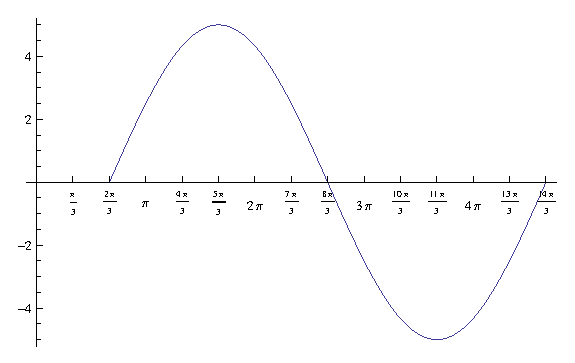
\includegraphics{graph1.eps}
            \caption{$f(x) = 5 \sin \left( \frac{1}{2} x - \frac{\pi}{3} \right)$}
          \end{figure}

        \end{solution}


        \question[10]
          Find the period and graph:
          \[
            f(x) = \cot \left( \pi x - \frac{\pi}{4} \right)
          \]

          \begin{solution}
            \[
              f(x) = \cot \left( \pi x - \frac{\pi}{4} \right) = \cot \left[ \pi \left( x - \frac{1}{4} \right) \right ]
            \]

            \begin{figure}[H]
              \centering
              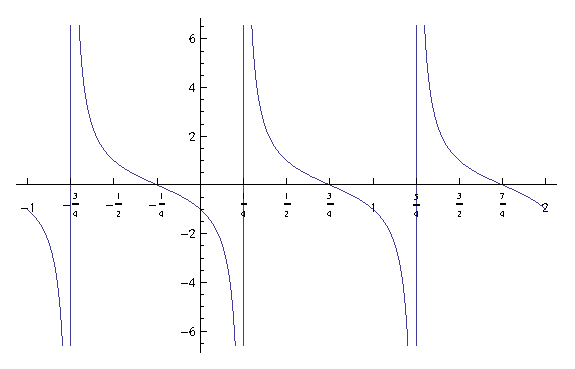
\includegraphics{graph2.eps}
              \caption{$f(x) = \cot \left( \pi x - \frac{\pi}{4} \right)$}
            \end{figure}

          \end{solution}

        \question[10]
        Find the period and graph:
          \[
            f(x) = 2 - 2 \sec x
          \]

          \begin{solution}
            \begin{figure}[H]
              \centering
              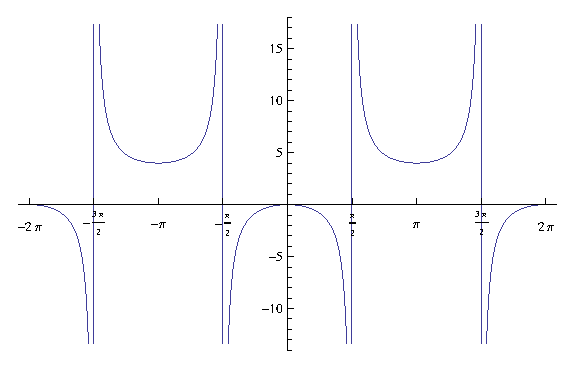
\includegraphics[scale=1.0]{graph3.eps}
              \caption{$f(x) = 2 - 2 \sec x $}
            \end{figure}

          \end{solution}

        \question[10]
          What is the equation for this graph?
          
          \begin{figure}[H]
            \centering
            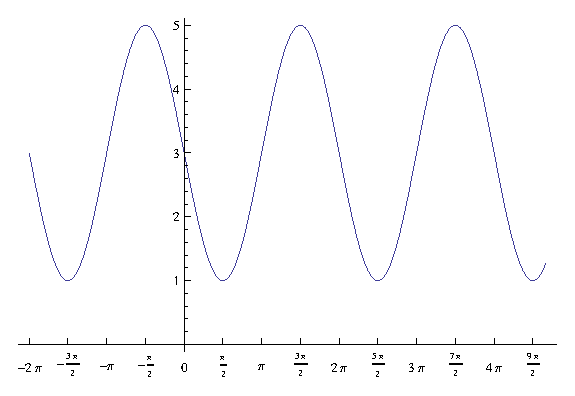
\includegraphics[scale=1.0]{graph4.eps}
            \caption{Find the equation}
          \end{figure}

          \begin{solution}
            \begin{itemize*}
              \item Since the graph goes between 1 and 5, the amplitude is 2.
              \item The zero point is shifted up by 3.
            \end{itemize*}

            You could think of the graph as either an inverted sine graph or a shifted cosine graph:
            \begin{align*}
              f(x) &= 3 - 2 \sin x \\
              g(x) &= 3 + 2 \cos \left( x + \frac{\pi}{2} \right) \\
            \end{align*}

          \end{solution}

          \question[10] Arthur Weasley's Flying Ford Anglia is hovering 1 foot off the ground.  The wheels have a radius
          of 9 inches and are spinning at a steady 3 revolutions per second.  Find an equation for the height in inches
          from the ground of a Cornish Pixie squashed on the bottom of one of the wheels.

          \begin{solution}
            \begin{itemize*}
              \item The angular velocity is: $\omega = 3 \cdot 2 \pi = 6 \pi$
              \item The offset is the height off the ground plus the radius or 21 inches.
              \item The amplitude is $\unit[9]{inches}$
            \end{itemize*}

            The equation is: $h(t) = 21 + 9 \sin 6 \pi t$ 

            \begin{figure}[H]
              \centering
              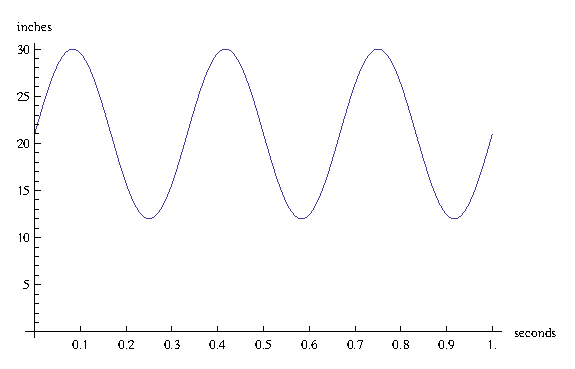
\includegraphics[scale=1.0]{graph5.eps}
              \caption{Cornish Pixie Height}
            \end{figure}

          \end{solution}

  \end{questions}
\end{document}

